\documentclass[journal,12pt,twocolumn]{IEEEtran}
\usepackage{setspace}
\usepackage{gensymb}
\singlespacing
\usepackage[cmex10]{amsmath}
\usepackage{amsthm}
\usepackage{mathrsfs}
\usepackage{txfonts}
\usepackage{stfloats}
\usepackage{bm}
\usepackage{cite}
\usepackage{cases}
\usepackage{subfig}
\usepackage{longtable}
\usepackage{multirow}
\usepackage{enumitem}
\usepackage{mathtools}
\usepackage{steinmetz}
\usepackage{tikz}
\usepackage{circuitikz}
\usepackage{verbatim}
\usepackage{tfrupee}
\usepackage[breaklinks=true]{hyperref}
\usepackage{graphicx}
\usepackage{tkz-euclide}
\usetikzlibrary{calc,math}
\usepackage{listings}
\usepackage{color}                                            %%
\usepackage{array}                                            %%
\usepackage{longtable}                                        %%
\usepackage{calc}                                             %%
\usepackage{multirow}                                         %%
\usepackage{hhline}                                           %%
\usepackage{ifthen}                                           %%
\usepackage{lscape}     
\usepackage{multicol}
\usepackage{chngcntr}
\DeclareMathOperator*{\Res}{Res}
\renewcommand\thesection{\arabic{section}}
\renewcommand\thesubsection{\thesection.\arabic{subsection}}
\renewcommand\thesubsubsection{\thesubsection.\arabic{subsubsection}}
\renewcommand\thesectiondis{\arabic{section}}
\renewcommand\thesubsectiondis{\thesectiondis.\arabic{subsection}}
\renewcommand\thesubsubsectiondis{\thesubsectiondis.\arabic{subsubsection}}
\hyphenation{op-tical net-works semi-conduc-tor}
\def\inputGnumericTable{}                                 %%

\lstset{
%language=C,
frame=single, 
breaklines=true,
columns=fullflexible
}
\begin{document}
\newtheorem{theorem}{Theorem}[section]
\newtheorem{problem}{Problem}
\newtheorem{proposition}{Proposition}[section]
\newtheorem{lemma}{Lemma}[section]
\newtheorem{corollary}[theorem]{Corollary}
\newtheorem{example}{Example}[section]
\newtheorem{definition}[problem]{Definition}
\newcommand{\BEQA}{\begin{eqnarray}}
\newcommand{\EEQA}{\end{eqnarray}}
\newcommand{\define}{\stackrel{\triangle}{=}}
\bibliographystyle{IEEEtran}
\raggedbottom
\setlength{\parindent}{0pt}
\providecommand{\mbf}{\mathbf}
\providecommand{\pr}[1]{\ensuremath{\Pr\left(#1\right)}}
\providecommand{\qfunc}[1]{\ensuremath{Q\left(#1\right)}}
\providecommand{\sbrak}[1]{\ensuremath{{}\left[#1\right]}}
\providecommand{\lsbrak}[1]{\ensuremath{{}\left[#1\right.}}
\providecommand{\rsbrak}[1]{\ensuremath{{}\left.#1\right]}}
\providecommand{\brak}[1]{\ensuremath{\left(#1\right)}}
\providecommand{\lbrak}[1]{\ensuremath{\left(#1\right.}}
\providecommand{\rbrak}[1]{\ensuremath{\left.#1\right)}}
\providecommand{\cbrak}[1]{\ensuremath{\left\{#1\right\}}}
\providecommand{\lcbrak}[1]{\ensuremath{\left\{#1\right.}}
\providecommand{\rcbrak}[1]{\ensuremath{\left.#1\right\}}}
\theoremstyle{remark}
\newtheorem{rem}{Remark}
\newcommand{\sgn}{\mathop{\mathrm{sgn}}}
%\providecommand{\abs}[1]{\left\vert#1\right\vert}
\providecommand{\res}[1]{\Res\displaylimits_{#1}} 
\providecommand{\norm}[1]{$\left\lVert#1\right\rVert$}
%\providecommand{\norm}[1]{\lVert#1\rVert}
\providecommand{\mtx}[1]{\mathbf{#1}}
\providecommand{\mean}[1]{E$\left[ #1 \right]$}
\providecommand{\fourier}{\overset{\mathcal{F}}{ \rightleftharpoons}}
%\providecommand{\hilbert}{\overset{\mathcal{H}}{ \rightleftharpoons}}
\providecommand{\system}{\overset{\mathcal{H}}{ \longleftrightarrow}}
%\newcommand{\solution}[2]{\textbf{Solution:}{#1}}
\newcommand{\solution}{\noindent \textbf{Solution: }}
\newcommand{\cosec}{\,\text{cosec}\,}
\providecommand{\dec}[2]{\ensuremath{\overset{#1}{\underset{#2}{\gtrless}}}}
\newcommand{\myvec}[1]{\ensuremath{\begin{pmatrix}#1\end{pmatrix}}}
\newcommand{\mydet}[1]{\ensuremath{\begin{vmatrix}#1\end{vmatrix}}}
\numberwithin{equation}{subsection}
\makeatletter
\@addtoreset{figure}{problem}
\makeatother
\let\StandardTheFigure\thefigure
\let\vec\mathbf
\renewcommand{\thefigure}{\theproblem}
\def\putbox#1#2#3{\makebox[0in][l]{\makebox[#1][l]{}\raisebox{\baselineskip}[0in][0in]{\raisebox{#2}[0in][0in]{#3}}}}
\def\rightbox#1{\makebox[0in][r]{#1}}
\def\centbox#1{\makebox[0in]{#1}}
\def\topbox#1{\raisebox{-\baselineskip}[0in][0in]{#1}}
\def\midbox#1{\raisebox{-0.5\baselineskip}[0in][0in]{#1}}
\vspace{3cm}
\title{EE3025-Assignment 1}
\author{Raagini Vishnubhotla - EE17BTECH11050}
\maketitle
\newpage
\bigskip
\renewcommand{\thefigure}{\theenumi}
\renewcommand{\thetable}{\theenumi}
Download all python codes from 
\begin{lstlisting}
https://github.com/raagini99/EE3025/tree/main/Assignment%201/codes
\end{lstlisting}
%
and latex-tikz codes from 
%
\begin{lstlisting}
https://github.com/raagini99/EE3025/tree/main/Assignment%201
\end{lstlisting}
\section{Problem}
5.3 The system h(n) is said to be stable if 
\begin{align}
\sum_{n=-\infty}^{\infty} \abs{|h(n)|} < \infty
\end{align} 
Is the system defined by (3.2) stable for impulse response in (5.1)?
\section{Solution}

\textbf{BIBO (Bounded-Input, Bounded-Output) Stability:}
A system is said to be BIBO stable, if the output of the system is bounded for every input to the system that is bounded, i.e.,
\begin{align}
    |x(n)|\leq B_x<\infty \implies |y(n)| \leq B_y<\infty
\end{align}

\textbf{Condition for BIBO Stability in Time Domain:}
Let the input $x(n)$ be bounded, i.e.,\\
\begin{align}
    |x(n)|\leq B_x<\infty
\end{align}
W.k.t.,\\
\begin{align}
    y(n)=\sum_{-\infty}^{\infty}h(k)x(n-k)
\end{align}
Applying modulus on both sides, we get\\
\begin{align}
    |y(n)|=|\sum_{-\infty}^{\infty}h(k)x(n-k)|\\
    \implies |y(n)| \leq |\sum_{-\infty}^{\infty}h(k) B_x|\\
    \implies |y(n)| \leq B_x|\sum_{-\infty}^{\infty}h(k)|
\end{align}
For the system to be BIBO stable, $|y(n)| < \infty$. This holds only if 
\begin{align}
    |\sum_{-\infty}^{\infty}h(k)| < \infty
\end{align}
i.e., for the system to be BIBO stable, it's impulse response in time domain must be absolutely summable.  
\\

\textbf{In given system,}\\
\begin{align}
    y(n)+\frac{1}{2}y(n-1) = x(n)+x(n-2) \\
    y(n)=0 \text{ for }n<0
\end{align}
Applying Z-transform on both sides,
\begin{align}
    Y(z) + \frac{1}{2}z^{-1}Y(z)=X(z) + z^{-2}X(z)\\
    \implies Y(z)=\frac{1+z^{-2}}{1+\frac{1}{2}z^{-1}}X(z)\\
    \implies \frac{Y(z)}{X(z)}=\frac{1+z^{-2}}{1+\frac{1}{2}z^{-1}}
\end{align}
But,
\begin{align}
    H(z) = \frac{Y(z)}{X(z)}
\end{align}
Plugging 2.0.13 into 2.0.12
\begin{align}
    \implies H(z) = \frac{1+z^{-2}}{1+\frac{1}{2}z^{-1}}\\
    \implies H(z) = \frac{1}{1+\frac{1}{2}z^{-1}} + \frac{z^{-2}}{1+\frac{1}{2}z^{-1}}
\end{align}
Applying inverse Z-transform on both sides, we get,
\begin{align}
\implies h(n)=\sbrak{\frac{-1}{2}}^nu(n) + \sbrak{\frac{-1}{2}}^{n-2}u(n-2)
\end{align}
Now checking if the system is BIBO stable using 2.0.7,
\begin{align}
    \sum_{n=-\infty}^{\infty}|\abs{\sbrak{\frac{-1}{2}}^nu(n) + \sbrak{\frac{-1}{2}}^{n-2}u(n-2)}| < \infty \\
    \implies \sum_{n=-\infty}^{\infty}|\abs{\sbrak{\frac{1}{2}}^nu(n) + \sbrak{\frac{1}{2}}^{n-2}u(n-2)}| < \infty \\
    \implies 2\sum_{n=-\infty}^{\infty}|\abs{\sbrak{\frac{1}{2}}^nu(n)}| < \infty \\
    \implies 2\sbrak{\frac{1}{1-\frac{1}{2}}} < \infty \\
    \implies 4 < \infty
\end{align}
which is true. Therefore, the system is BIBO stable.\\ 
\\
\textbf{Additional:}\\
When h(n) is absolutely summable, i.e.,
\begin{align}
    \sum_{n=-\infty}^{\infty} |\abs{h(n)}|  &< \infty \\
    \sum_{n=-\infty}^{\infty}\abs{|h(n)z^{-n}|}_{|\abs{z}|=1}&<\infty \\
\end{align}
From triangle inequality,
\begin{align}
    \abs{|\sum_{n=-\infty}^{\infty}h(n)z^{-n}|}_\abs{|z|=1}<\sum_{n=-\infty}^{\infty}\abs{|h(n)z^{-n}|}_{\abs{|z|}=1}
\end{align}
Plugging 2.0.25 into 2.0.24, we get, 
\begin{align}
    \implies \abs{|H(z)|}_{\abs{|z|}=1}&<\infty 
\end{align}

Therefore, the Z transform of the system's ROC includes the unit circle. \\
\begin{align}
    H(z) = \frac{1+z^{-2}}{1+\frac{1}{2}z^{-1}} \\
    H(z) = \frac{2(z^2+1)}{z(2z+1)} 
\end{align}
Solving, we get, \\
\begin{align}
    Poles = 0 , -\frac{1}{2} \\
    Zeros = +1j, -1j
\end{align}

\begin{figure}[h!]
    \centering
    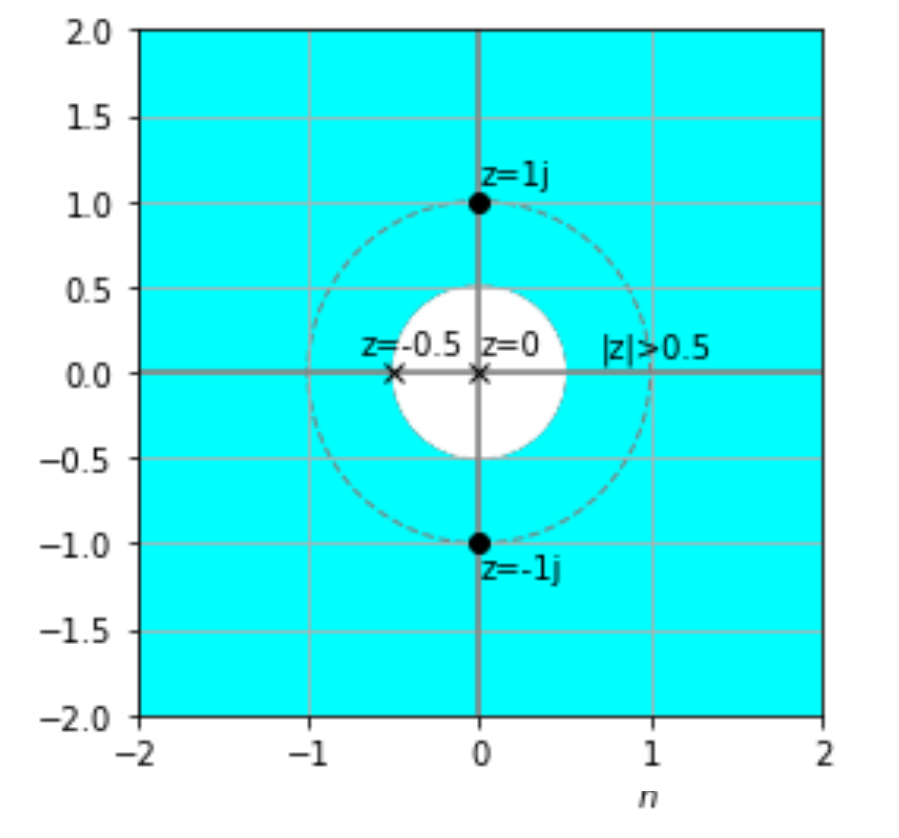
\includegraphics[width=8cm]{asst_1_img_3.png}
    \caption{Pole-Zero Plot}
\end{figure}\\
Therefore, from the solved equations or Z plane plot, the same is verified. \\

\textbf{Verification of BIBO stability of given system for an example:} \\
Given system: 
\begin{align}
    y(n)+\frac{1}{2}y(n-1) = x(n)+x(n-2) \\
    y(n)=0 \text{ for }n<0
\end{align}
Let input be given as follows:
\begin{align}
    x(n)=\{1,2,3,4,2,1\}
\end{align}
\begin{figure}[h!]
    \centering
    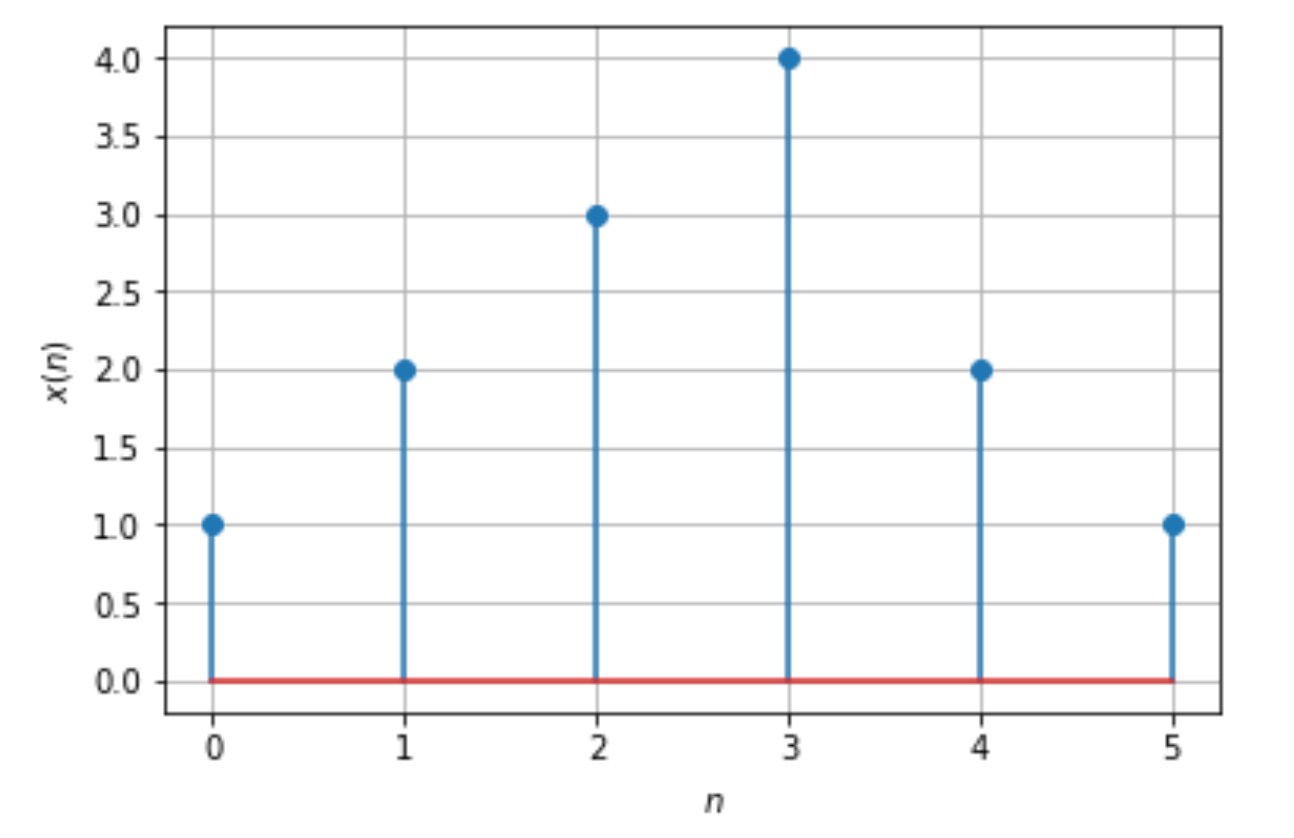
\includegraphics[width=8cm]{asst_1_img_1.png}
    \caption{Input signal, x(n)}
\end{figure}
$B_x=4$ for the input signal. \\
Passing the signal through the system, we get the following signal: \\
\begin{figure}[h!]
    \centering
    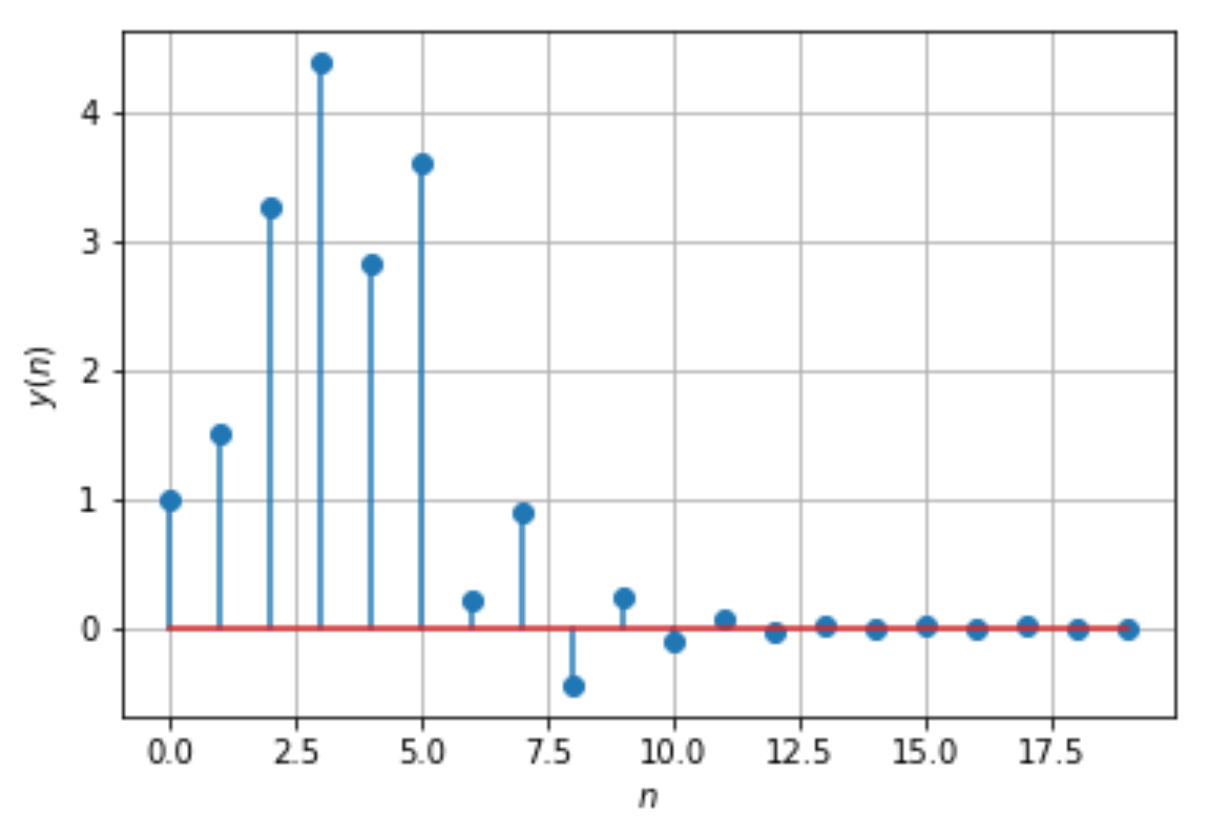
\includegraphics[width=8cm]{asst_1_img_2.png}
    \caption{Output signal, y(n)}
\end{figure}
$B_y=4.375$ for the output signal. \\
Therefore, since the system is BIBO stable, \\
$B_x< \infty \implies B_y< \infty $
\end{document}